\documentclass[12pt,tightenlines,letterpaper]{scrartcl}
\usepackage{lmodern}
\usepackage{ifxetex,ifluatex}
\usepackage{fixltx2e} % provides \textsubscript
\ifnum 0\ifxetex 1\fi\ifluatex 1\fi=0 % if pdftex
  \usepackage[T1]{fontenc}
  \usepackage[utf8]{inputenc}
\else % if luatex or xelatex
  \ifxetex
    \usepackage{mathspec}
  \else
    \usepackage{fontspec}
  \fi
  \defaultfontfeatures{Ligatures=TeX,Scale=MatchLowercase}
\fi

%%% Needed to write listtodonotes, and listofalgorithms, but the problem is listoftodonotes
% \usepackage{morewrites}
\usepackage[
HomeHTMLFilename=index,     % Filename of the homepage.
%HTMLFilename={node-},       % Filename prefix of other pages.
%IndexLanguage=english,      % Language for xindy index, glossary.
latexmk,                    % Use latexmk to compile.
%   OSWindows,                  % Force Windows. (Usually automatic.)
mathjax,                    % Use MathJax to display math.
]{lwarp}


\title{Block Chain Notes}
\author{David Li}
\setcounter{tocdepth}{2} % Include subsections in the \TOC.
\setcounter{secnumdepth}{2} % Number down to subsections.
\setcounter{FileDepth}{0} % Split \HTML\ files at sections, in this case chapters?, 0 for chapters?
\booltrue{CombineHigherDepths} % Combine parts/chapters/sections
\setcounter{SideTOCDepth}{1} % Include subsections in the side\TOC
\HTMLAuthor{David Li} % Sets the HTML meta author tag.
\HTMLLanguage{en-US} % Sets the HTML meta language.
\HTMLDescription{A list of cheatsheets for courses at the University of Victoria}% Sets the HTML meta description.
\HTMLFirstPageTop{ CheatSheets \fbox{
\includegraphics[width=1\linewidth]{Images/Ethereum-Cover.png}}}
\HTMLPageTop{\fbox{
\includegraphics[width=1\linewidth]{Images/Ethereum-Cover.png}}}
\HTMLPageBottom{Made by David Li}
\newcommand{\printTitle}{Insert a title Here} 
\usepackage{graphicx} % Required for including pictures
\graphicspath{{Images/}} % Specifies the directory where pictures are stored

%%%% Useful Packages loaded without much configuration %%%%%%
\usepackage[margin=2.54 cm]{geometry} % Set dimensions for page layout
\usepackage{kpfonts}	    % Fonts used in the title page
\usepackage{eso-pic}        % Background pictures in the title page
\usepackage{tcolorbox}		% Fancy Math equations	
\usepackage{tabularx}		% Tabulars with adjustable-width columns
\tcbuselibrary{skins} 	% used with tcolorbox 
\usepackage{transparent}	% Create transparent background images
\usepackage{lipsum}  % Garbage text
\usepackage{url}	 % links to websites
\usepackage{pdfpages} % to include pdf pages
\usepackage{booktabs}	% Make high quality tables
\usepackage{colortbl}	% Color tables
\usepackage{xfrac}		% Make fractions nice in tables
\usepackage{enumitem}	% itemize, enumerate
\usepackage{array}
\usepackage{setspace}   % double spacing as required in UVIC co-op reports
\usepackage{titlesec} % Select alternative section titles
\titlespacing*{\section}
{0pt}{5.5ex plus 1ex minus .2ex}{4.3ex plus .2ex}	% Not sure about this spacing
\usepackage{multirow} % Create tabular cells spanning multiple rows.

\usepackage{float}    % used for float­ing ob­jects such as fig­ures and ta­bles.
\usepackage{caption}
%\captionsetup[figure]{labelfont=sf,textfont={sf}}
%\captionsetup[table]{labelfont=sf,textfont={sf}}
% \usepackage{parskip} % no indents, don't use in lwarp
\usepackage{tikz}	 % for drawings and cool graphics

%% Math packages %%
\usepackage{siunitx}	% SI units
\usepackage{mathtools}	% LOAD MATH
\usepackage{amssymb}  	% MATH Symbols


%%%%%%%%%% COLORS %%%%%%%%%%%%%%%%%%%%%%%%%%%%%
\definecolor{titlepagecolor}{cmyk}{1,.60,0,.40}

%%%%%%%%%%%%%%%%%%%%%%%%%%%%%%%%%%%%%%%%%%%%%%%%%%%%%%%%%%%%%%%%%%%%%%
%%%%%%%%%%%%%%%%%%%%%%%%%%%% CODE STYLINGS %%%%%%%%%%%%%%%%%
%%%%%%%%%%%%%%%%%%%%%%%%%%%%%%%%%%%%%%%%%%%%%%%%%%%%%%%%%%%%%%%%%%%%%%%%

\usepackage{listings} % For source code
\DeclareCaptionFont{white}{\color{white}}
\DeclareCaptionFormat{listing}{\colorbox{titlepagecolor}{\parbox{1\textwidth}{#1#2 \quad #3}}}
\captionsetup[lstlisting]{format=listing,labelfont=white,textfont={white,sf}} % for fancy boxes

\lstdefinestyle{default}{frame=tb,
	aboveskip=3mm,
	backgroundcolor=\color{cornsilk},
	belowskip=3mm,
	showstringspaces=false,
	columns=flexible,
	basicstyle={\ttfamily},
	numbers=none,
	numberstyle=\tiny\color{red},
	keywordstyle=\color{blue},
	commentstyle=\color{green},
	stringstyle=\color{purple},
	morekeywords={fclose, exit, printf, fscanf, strcpy, strlen,
		strcmp, fprintf},
	breaklines=true,
	breakatwhitespace=true,
	tabsize=3,
	captionpos=t,
	columns=flexible,
}
%%%%%%%%%%%%%%%%%%%%%%%%%%%%%%%
%%%%%% SQL style setup %%%%%%%%
\makeatletter
\newcommand{\lstuppercase}{\uppercase\expandafter{\expandafter\lst@token
		\expandafter{\the\lst@token}}}	%%%UPPERCASE SQL%%%%
\newcommand{\lstlowercase}{\lowercase\expandafter{\expandafter\lst@token
		\expandafter{\the\lst@token}}} %%% REGULAR CASE %%%%
\makeatother

\definecolor{mauve}{rgb}{0.58,0,0.82}
\lstdefinestyle{Oracle}{basicstyle=\ttfamily,
	keywordstyle=\lstuppercase,
	backgroundcolor=\color{cornsilk},
	emphstyle=\itshape,
	showstringspaces=false,
	morekeywords={ACCESS, MOD, NLS_DATE_FORMAT, NVL, REPLACE, SYSDATE,
		TO_CHAR, TO_NUMBER, TRUNC},
	numberstyle=\tiny\color{black},
	keywordstyle=\color{red},
	commentstyle=\color{green},
	stringstyle=\color{mauve},
	columns=flexible,
}
%%%%%%%%%%%%%%%%%%%%%%%%%%%%%%%%%%%%%%%%%%%%%%%%
%%%%%%%%%%%%%%%%%%%%%JAVA %%%%%%%%%%%%%%%%%%%%%%
\definecolor{javared}{rgb}{0.6,0,0} % for strings
\definecolor{javagreen}{rgb}{0.25,0.5,0.35} % comments
\definecolor{javapurple}{rgb}{0.5,0,0.35} % keywords
\definecolor{javadocblue}{rgb}{0.25,0.35,0.75} % javadoc
\lstdefinestyle{myJava}{frame=tb,
	basicstyle=\ttfamily,
	backgroundcolor=\color{cornsilk},
	keywordstyle=\color{javapurple}\bfseries,
	stringstyle=\color{javared},
	commentstyle=\color{javagreen},
	morecomment=[s][\color{javadocblue}]{/**}{*/},	% Make comments blue
	morecomment=[is]{/*}{*/},  % Remove comments
	stepnumber=2,
	numbers=left,    % print line numbers
	numbersep=10pt,
	tabsize=4,
	showspaces=false,
	showstringspaces=false,
	linewidth=\textwidth,
	columns=flexible,			% Important for keeping text in the frame
	breaklines=true,
}

%%%%%%%%%%%%%%%%%% ENDJAVA %%%%%%%%%%%%%%%%%%%%%
%%%%%%%%%%%%%%%%%%%%%%%%%%%%%%%%%%%%%%%%%%%%%%%%

%%%%%%%%%%%%%%%%%%%%%%%%%%%%%%%%%%%%%%%%%%%%%%%%%%
%%%%%%%%%%%%%%%%%%%%% JAVASCRIPT%%%%%%%%%%%%%%%%%%%
\lstdefinelanguage{JavaScript}{frame=tb,
	keywords={typeof, new, true, false, catch, function, return, null, catch, switch, var, if, in, while, do, else, case, break},
	keywordstyle=\color{blue}\bfseries,
	ndkeywords={class, export, boolean, throw, implements, import, this},
	ndkeywordstyle=\color{darkgray}\bfseries,
	identifierstyle=\color{black},
	sensitive=false,
	comment=[l]{//},
	morecomment=[s]{/*}{*/},
	commentstyle=\color{purple}\ttfamily,
	stringstyle=\color{red}\ttfamily,
	morestring=[b]',
	morestring=[b]"
}
\definecolor{cornsilk}{rgb}{1.0, 0.97, 0.86}
\lstdefinestyle{myJavaScript}{
	language=JavaScript,
	backgroundcolor=\color{cornsilk},
	extendedchars=true,
	basicstyle=\ttfamily,
	showstringspaces=false,
	showspaces=false,
	tabsize=2,
	breaklines=true,
	showtabs=false,
	captionpos=t,
}
%%%%%%%%%%%%%%%%%%%%%%%%%%%%%%%%%%%%%%%%%%%%%%%%%%
%%%%%%%%%%%%%% END CODE STYLINGS %%%%%%%%%%%%%%%%%
%%%%%%%%%%%%%%%%%%%%%%%%%%%%%%%%%%%%%%%%%%%%%%%%%

%%%%%%%%%%%%%%%%%%%%%%%%%%%%%%%%%%%%%%%%%%%%%%%%%%%%%%%%%%%%
%%%%%%%%%%%%%%%%%%%%%%%%% FORMATTING %%%%%%%%%%%%%%%%%%%%%%%
% Format TOC, header, footers and chapters
%% tocloft settings
\usepackage[titles]{tocloft}	% Pro­vides con­trol over the ty­pog­ra­phy of the Ta­ble of Con­tents, List of Fig­ures and List of Tables
\setlength{\cftbeforesecskip}{3pt}
% End tocloft settings

\usepackage{sectsty} % used to color chapter and sections
%\renewcommand{\cftpartleader}{\cftdotfill{\cftdotsep}} % for parts
%\renewcommand{\cftchapleader}{\cftdotfill{\cftdotsep}} % for chapters
\renewcommand{\cftsecleader}{\cftdotfill{\cftdotsep}} % for sections, if you really want! (It is default in report and book class (So you may not need it).
% ----------------------------------------------------------------
%\renewcommand{\cftdotsep}{0}	 % dots in the title page
% \renewcommand{\cftsectleader}{\bfseries\cftdotfill{\cftsecdotsep}}% dot leaders in bold 


   % NUMBERING IN TOC FOR SUMMARY SECTION %%%%%%%%
   \newcommand{\mysection}[2]{
   	\setcounter{section}{#1}
   	\setcounter{subsection}{0}
   	\section*{#2}
   	\addcontentsline{toc}{section}{#2}
   }
  
   %%%%%%%%%%%%%%%%%%%%%%%%%%%%%%%%
    %CHAPTER Title formatting
	\definecolor{myText}{HTML}{2B2B2B}
	\definecolor{myChap}{HTML}{000066}
	\definecolor{mySect}{HTML}{336699}
	\definecolor{mySubSect}{HTML}{2088B2}

    \renewcommand{\sectionmark}[1]{\markboth{\thesection.\ #1}{}}
    
    % SET UP COLOURS FOR HEADINGS IN THE REPORT
    \sectionfont{\color{mySect}}  % sets colour of sections
    \subsectionfont{\color{mySubSect}}  % sets colour of subsections
    \subsubsectionfont{\color{mySubSect}}  % sets colour of subsubsections
    \subparagraphfont{\color{red}}		    % sets colour of paragraphs

   	%%%%%%%%%%%%%%%%%%%%%%%%%%%%%%%%%%%%%%%%%%%%%%%%%%%%%%%%%%%%%%%%
   	%CHANGE  GLOBAL TEXT COLOR %%%%%%%%%%%%%%%%%%%%%
   	\makeatletter
   	\newcommand{\globalcolor}[1]{%
   		\color{#1}\global\let\default@color\current@color
   	}
   	\makeatother
   	
   	% Edit the global text colour, make the report easier to read for digital screens or print.
   	%\AtBeginDocument{\globalcolor{myText}}
   	
   %%%%%%%%%%%%%%%%%%%%%%%%%%%%%%%%%%%%%%%%%%%%%%%%%%%%%%%
   % SET UP COMBINED LOT and LOF 	%%%%%%%
   %	CONFIG LOL					%%%%%%%
   %%%%%%%%%%%%%%%%%%%%%%%%%%%%%%%%%%%%%%%%%%%%%%%%%%%%%%%%%%%
%   \makeatletter
%   \def\ext@figure{lot}
%   \makeatother\

%	\setcounter{tocdepth}{4} % INCLUDE SUBSUBSECTIONS IN TOC
  % \renewcommand{\lstlistingname}{Listing}	% Change caption in code listing
   %\renewcommand{\lstlistlistingname}{List of Scripts}     % CHANGE THE HEADER IN TOC
   
   % Create List of Figures and Tables in LATEX
%   \renewcommand*\listtablename{List of Figures and Tables}
%   \renewcommand{\cftfigpresnum}{Figure~}
%   \renewcommand{\cftfigaftersnum}{:}
%   \setlength{\cftfignumwidth}{5.5em}
%   \renewcommand{\cfttabpresnum}{Table~}		
%   \renewcommand{\cfttabaftersnum}{:}
%   \setlength{\cfttabnumwidth}{5.5em}
   
%   %CONFIG SCRIPTS in TOC %%%%%%
%   \makeatletter
%   \AtBeginDocument{%	Add the word Program in front of the caption in TOC and listing
%   	\renewcommand\lstlistoflistings{\bgroup
%   		\let\contentsname\lstlistlistingname
%	\def\l@lstlisting##1##2{\@dottedtocline{1}{1.3em}{3em}{\bfseries Script 
%				##1}{##2}}
%   		\let\lst@temp\@starttoc \def\@starttoc##1{\lst@temp{lol}}%
%   		\tableofcontents \egroup}
%   }
%   \makeatother
%   
%   %MAKE SPACING THE SAME AS IN THE LOT AND LOF in Programs %%%%%%
%%   \makeatletter
%%   \let\my@chapter\@chapter
%%   \renewcommand*{\@chapter}{%
%%   	\addtocontents{lol}{\protect\addvspace{10pt}}%
%%   	\my@chapter}
%%   \makeatother
   
%%%%%%%%%%%%%%%%%%%%%%%%%%%%%%%%%%%%%%%%%%%%%%%%%%%%%%%%%%%%%%%%%%
%%%%%% SET UP BIBLIOGRAPHY  %%%%%%%%%%%%%%%%%%%%%%%%%%%%%%%%%%%%%%%%%%%
%%%%%%%%%%%%%%%%%%%%%%%%%%%%%%%%%%%%%%%%%%%%%%%%%%%%%%%%%%%%%%%%%%
% See https://tex.stackexchange.com/questions/6967/how-to-split-bibliography-into-works-cited-and-works-not-cited?noredirect=1&lq=1
% https://tex.stackexchange.com/questions/128959/multiple-bibiographies-using-biblatex-and-resetting-numbers
\usepackage[defernumbers=true,backend=bibtex,sorting=none]{biblatex}	% Sort by citation order
\DeclareBibliographyCategory{cited}
\AtEveryCitekey{\addtocategory{cited}{\thefield{entrykey}}}
\defbibheading{bibliography}[\bibname]{%
  	\subsubsection*{#1}}%	% set up bibliography as a section 
  	%\markboth{\thesection.\ #1}{}}	%label at upper right corner in header

\usepackage[titletoc]{appendix}	%% appendix will be in the toc
% What I want is References and subsections or paragraphs 

% This created 5. Cited References and 6. General References
%\usepackage[nottoc,numbib]{tocbibind}	% Label the Biblography in the TOC
%\defbibheading{bibliography}[\bibname]{%
%  	\section{#1}%	% set up bibliography as a section 
%  	\markboth{\thesection.\ #1}{}}	%label at upper right corner in header
\newcommand{\onlineCite}{[Online] Available: }	% Used in BIBLIOGRAPHY
% Load all references 
\nocite{*}

%%%%%%%%%%%%%%%%%%%%%%%%%%%%%%%%%%%%%%%%%%%%%%%%%%%%%%%%%%%%%%%%%%%
%%%%%%%%% CUSTOMIZE GLOSSARY %%%%%%%%%%%%%%%%%%%%%%%%
\usepackage[toc,nopostdot,xindy]{glossaries} % included in toc and keep track of technical words and definition and remove dots at the end

% glossary definitions as bold
%\defglsentryfmt{\color{black}\bfseries\glsgenentryfmt}

% custom glossary style that contains the pages that contains the glossary terms, and bolded glossary entries.
%\newglossarystyle{myGloss}{%
%	\setglossarystyle{list}
%	\renewcommand*{\glossentry}[2]{%
%		\item[\textbf{\glsentryitem{##1}}%
%		\textbf{\glstarget{##1}}{\textbf{\glossentryname{##1}:}}]
%		\glossentrydesc{##1}\glspostdescription\space See p.\space ##2} 
%}
%\setglossarystyle{listhypergroup}
%\setglossarystyle{myGloss}

% Set up roman numercals page numbering for front matter, letter of transmittal, and table of contents.
% Commentout for lwarp
\newcommand\frontmatterNumbering{%
	\cleardoublepage
	%\@mainmatterfalse
	\pagenumbering{roman}}
\renewcommand{\familydefault}{\sfdefault} % Nice font formatting

\let\cleardoublepage\clearpage % prevent book from create extra pages bewteen chapters

%%% Set up verbatim for WYSIWYG formatting for letter
\usepackage[T1]{fontenc}%  selects EC fonts
\usepackage{verbatim}%     configurable verbatim
\makeatletter
\def\verbatim@font{\normalfont% select the font
	\let\do\do@noligs
	\verbatim@nolig@list}
\makeatother



%%%% Set up headers %%%%
\usepackage{fancyhdr}	% Controls headers and footers
   \fancypagestyle{plain}{
   	\fancyhf{}
   	\setlength{\headheight}{15pt} 
   	\fancyhead[L]{ \textsf{Creating transparent and efficient transactions through smart contracts and blockchain}}
   	%\fancyhead[R]{\textsf{\leftmark}}
   	\fancyfoot[C]{\textsf{ENGR 446: Technical Report}}
   	\fancyfoot[L]{\textsf{David Li}}
   	\fancyfoot[R]{\textsf{\thepage}}
   	\renewcommand{\headrulewidth}{0.4pt}
   	\renewcommand{\footrulewidth}{0.4pt}
   }
   
    % NUMBERING IN TOC FOR SUMMARY SECTION %%%%%%%%
      \newcommand{\mychapter}[2]{
      	\setcounter{chapter}{#1}
      	\setcounter{section}{0}
      	\chapter*{#2}
      	\addcontentsline{toc}{chapter}{#2}
      }
     
      %%%%%%%%%%%%%%%%%%%%%%%%%%%%%%%%
      % Remove Footer on select pages
      \fancypagestyle{nofooter}{%
      	\fancyfoot{}%
      	\fancyhead{}%
      }

% Diagram, adjust big picture
\usepackage{adjustbox}

%\usepackage[x11names,table]{xcolor}
%\DeclareCaptionFont{blue}{\color{LightSteelBlue3}}

\newcommand{\foo}{\color{blue}\makebox[0pt]{\textbullet}\hskip-0.5pt\vrule width 1pt\hspace{\labelsep}}



%%% Following lwarps documentation hyperref will be loaded last
%CHANGE Link colours as needed
\definecolor{linkColor}{HTML}{453737}	

\usepackage{hyperref}	% Create links in document
\hypersetup{linktocpage}	% Allow clickable links
\hypersetup{
    bookmarks=true,         % show bookmarks bar?
    unicode=false,          % non-Latin characters in Acrobat’s bookmarks
    pdftoolbar=true,        % show Acrobat’s toolbar?
    pdfmenubar=true,        % show Acrobat’s menu?
    pdffitwindow=false,     % window fit to page when opened
    pdfstartview={FitH},    % fits the width of the page to the window
    pdftitle={ENGR 446: Smart Contracts},    % title
    pdfauthor={David Li},     % author	
    %linktoc=all,     %set to all if you want both sections and subsections linked
	colorlinks   = true, %Colours links instead of ugly boxes
	urlcolor     = blue, %Colour for external hyperlinks
	linkcolor    = blue, %Colour of internal links
	citecolor   = black %Colour of citations
}
%%%%%%%%%%%%%%%%%%%%%%%%%%%%%%%%%%%%%%%%%%%%%%%%%%
%%%%%%%%%%% END PREAMBLE %%%%%%%%%%%%%%%%%%%%%%%%%
%%%%%%%%%%%%%%%%%%%%%%%%%%%%%%%%%%%%%%%%%%%%%%%%%%
\addbibresource{references.bib}	% Load bibliography
%% LaTeX2e file `glossary.tex'
%% generated by the `filecontents' environment
%% from source `reportContent' on 2018/07/28.
%%
\newglossaryentry{sql}
{
 name={SQL},
 description={SQL (Structured Query Language) is a standard interactive and programming language for getting information from and updating a database.},
 first={Structured Query Language (SQL)},
 long={Structured Query Language}
}
\newglossaryentry{sd}
{
 name={System Documentation},
 text={documentation},
 description={A collection of documents that describes the requirements, \newline capabilities, limitations, design, operation, and maintenance of a system, such as a communications, computing, or information processing system.},
 long={System Documentation}
}

\newglossaryentry{sharepoint}
{
 name={SharePoint},
 description={A browser-based collaboration and document management platform from Microsoft. },
 first={Microsoft SharePoint},
 long={Microsoft Lync}
}
\newglossaryentry{JIRA}
{
 name={JIRA},
 description={Software development tool  that is mainly used for bug tracking and project management by \gls{agile} teams. },
}
\newglossaryentry{agile}
{
 name={agile},
 description={Iterative approach to software delivery that creates software incrementally from the beginning of the project, instead of trying to deliver it all at once near the end.},
}
\newglossaryentry{scrum}
{
 name={Scrum},
 description={Scrum is an iterative and incremental agile software development framework for managing product development.}
}
\newglossaryentry{kanban}
{
 name={Kanban},
 description={Kanban is a method for managing knowledge work which balances the demand for work to be done with the available capacity to start new work.}
}
\newglossaryentry{Confluence}
{
 name={Confluence},
 description={Team collaboration software which allows team members to create, share and collaborate information.},
}

\newglossaryentry{jql}
{
 name={JQL},
 description={Structured queries to search for issues in JIRA. It is the most flexible way to search for issues in JIRA and similar to \gls{sql} },
 first={JIRA Query Language (JQL)},
 long={JIRA Query Language}
}
\newglossaryentry{excel}
{
 name={Excel},
 description={Electronic Spreadsheet Program that is used for storing, organizing and manipulating data.},
 first={Microsoft Excel},
 long={JIRA Query Language}
}
\newglossaryentry{MOTI}
{
 name={MOTI},
 description={Previous Employeer},
 first={INSERT PREVIOUS EMPLOYEER},
 long={Previous Employeer}
}
\newglossaryentry{IMB}
{
 name={IMB},
 description={Infomration DIVIOSN},
 long={Infomration DIVIOSN},
 first={IInfomration DIVIOSN}
}
\newglossaryentry{wiki}
{
 name={wiki},
 description={a website that allows collaborative editing of its content and structure by its users.}
}
\newglossaryentry{ssot}
{
 name={single source of truth},
 description={one source of data that everyone in a organization agrees is the real, trusted number for some operating data.}
}
\newglossaryentry{issue}
{
 name={issue},
 description={unit of work to accomplish an improvement in a system such as access requests and tasks.}
}

\makeglossaries
\linespread{1.25}
% Reason: the standard line skip means a factor of 1.2 (such as font height 10pt, base line skip 12pt). Multiply with \linespread, so you get 1.25*1.2 = 1.5, so one-half.

\renewcommand{\printTitle}{Determining Potential Uses of JIRA and Confluence}

\begin{document}
%% Use roman numercals page numbering for front matter, letter of transmittal, and table of contents.
\frontmatterNumbering

% Manually modified the word front page template, and then save to pdf and include using includepdf.
%\includepdf{TitlePage.pdf}
%%%% Add the required double spacing %%%
%%% LETTER OF TRANMISSAL %%%%
 \linespread{1}
 \begin{verbatim}
 Insert Title of Report Here
 ENGR 446
 4A Computer Engineering 
 Dr Helen Bailey
 Faculty of Engineering
 University of Victoria
 P.O. Box 1700
 Victoria, B.C.
 V8W 2Y2
 
 Dear Helen, 
 
 Please accept the accompanying ENGR 446 Final Technical Report entitled "Creating transparent and efficient transactions through smart contracts and blockchain."
 
 This report is the result of interest and exposure to blockchain development and technologies as part of my third co-op work term. Using the most popular smart contract programming language, Solidity, I created logic for a decentralized application. Some issues of implementing and determinating the viability of smart contracts to simplify transactions include regulation, conflict resolvement and ability to reverse fraduent transactions. Technological advances including exponential increases in computational power 
 that would render the blockchain unsecure are not explored. Some problems faced in this report include rapid changes in technology, constantly changing standards, and legal uncertainty surrounding blockchain.
 
 I would like to thank my manager, Dino Coletti, for his patience and good judgement, as well as
 the my coworkers who were always willing to help.
 
 Sincerely,

 \end{verbatim}
 \fancyhf{} % sets both header and footer to nothing
% \thispagestyle{nofooter}	% Don't print page number in footer
%%%%%%%%%%%%%%%%%%%%%%%%%%%%%%%%%%%%%%%%%%%%%%%%%%%%%%%%%%%%%%%%%
%%%%%%%%%%%%%%%%%%%%%% TABLE OF CONTENTS %%%%%%%%%%%%%%%%%%%%%%%%%
%%%%%%%%%%%%%%%%%%%%%%%%%%%%%%%%%%%%%%%%%%%%%%%%%%%%%%%%%%%%%%%%%%
% Stop page breaks for list of figures and list of tables
%{\listoffigures \let\cleardoublepage\clearpage \listoftables}

\begingroup
\cleardoublepage
\phantomsection

%\setcounter{tocdepth}{0}  0 means only chapters in toc, 1 includes sections, 2 includes subsections, etc.

\renewcommand{\contentsname}{Table of Contents}
\tableofcontents   % Print table of contents
\cleardoublepage %\cleardoublepage %for openright
\listoffigures					  %List of Figures
\phantomsection
\listoftables					  %List of Tables

\clearpage
\lstlistoflistings				  %List of Code listings
%\addcontentsline{toc}{section}{{Listings}}	% ADD HEADING TO TOC
\endgroup
%%%%%%%%%%%%%%%%%%%%%%%%%%%%%%%%%%%%%%%%%%%%%%%%%%%%%%%%%%%%%%%%%
%%%%%%%%%%%%%%%%%%%%%% END TABLE OF CONTENTS %%%%%%%%%%%%%%%%%%%%%%%%%
%%%%%%%%%%%%%%%%%%%%%%%%%%%%%%%%%%%%%%%%%%%%%%%%%%%%%%%%%%%%%%%%%%

%%%%%%%%%%%%%%%%%%%%%%%%%%%%%%%%%%%%%%%%%%%%%%%%%%%%%%%%%%%%%
%%%%%%%%%%%%%% SUMMARY %%%%%%%%%%%%%%%%%%%%%%%%%%%%%%%%%%%%%%
%%%%%%%%%%%%%%%%%%%%%%%%%%%%%%%%%%%%%%%%%%%%%%%%%%%%%%%%%%%%%


  \section*{Summary } 
  \addcontentsline{toc}{section}{Summary} % Manually add the unlabelled section, summary is not numbered as specified in university co-op report standards.
  The rise of centralized music streaming platforms has significantly reduced artist compensation because incentives to pay music labels first, unclear payment structures, and a lack of transparency. Another way to compensate artists is to issue digital tokens, which are spendable on accommodations, recording time and studio time. In order to empower artists and avoid pitfalls of streaming services, ownership and control of digital token must be decentralized. %however, implementation of a decentralized application can increase tra
   
   Although \gls{blockchain} is the technology that is associated with the cryptocurrency, Bitcoin, the use cases of blockchain are numerous including building decentralized applications. Ensuring that digital assets can be redeemed requires the usage of \glspl{smart contract} to automatically execute transactions. Additionally, ensuring ownership of tokens and safe transfers of digital assets are essential.
   
   Visually representation of rewards can be implemented using an image, hosted of decentralized storage such as IPFS, or contain a form of "dna" that maps to specific components.
 %As dependencies on e-commerce increase and  
 %In the continuing effort to 
 %In the continuing effort to organize high-quality reliable information, the %\gls{MOTI} \gls{IMB} is presently experimenting with \gls{JIRA}, an \gls{issue} tracking tool and \gls{Confluence}, \gls{wiki} software for technical documentation. Although good quality information is critical to operations, \gls{sd} is inconsistent and scattered across multiple sources, some of which require access permissions.\gls{JIRA} and Confluence are software tools that improve productivity and organization within MOTI IMB. \\ \\
 %Benefits from connecting \gls{JIRA} and \gls{Confluence} include common user management, reporting on existing JIRA \glspl{issue} in \gls{Confluence} and switching between application quickly. Extending the functionality of these tools by installing add-ons will assist in improving \gls{sd}. Purchasing software such as \gls{Confluence} to solve the \gls{sd} problem is inadequate because software can be poorly designed or implemented. These software tools assist in information management, but full utilization and proper implementation is required to improve documentation.
 
 % Uncomment to enable double spacing %
 % \doublespacing

%%%%%%%%%%%%%%%%%%%%%%%
%%%%% GLOSSARY %%%%%%%%
%%%%%%%%%%%%%%%%%%%%%%%
% Alternative usage of glossary
%\printglossary[title=List of Terms,toctitle=Terms and abbreviations] 
\newpage
 \printglossaries	%%% PRINT GLOSSARIES %%%%
 \clearpage 
 
 
 %%% Set page numbers for introduction %%
\addtocounter{section}{0}	%%% start at page #1 Introduction.
\setcounter{page}{1}% Start page number with 1
\renewcommand{\thepage}{\arabic{page}}% Arabic numerals for page counter
%%%%%%%%%%%%%%%%%%%%%%%%%%%%%%%%%%%%%%%%%%%%%%
%%%% Inserting Main Content %%%%%%%%%%%%%%%%%%%
%%%%%%%%%%%%%%%%%%%%%%%%%%%%%%%%%%%%%%%%%%%%%%
\pagestyle{plain}
\section{Introduction}

\subsection{Background}
\subsubsection[Overview]{History of Cryptocurrency}
\vspace*{-0.5cm}

\begin{minipage}[h]{0.45\linewidth}
%Print version of table
\begin{warpprint}
\begin{table}[H]
\centering
\renewcommand\arraystretch{1.4}\arrayrulecolor{blue}
\captionsetup{singlelinecheck=false, labelfont=sc, labelsep=quad}
\caption{Timeline of Cryptocurrency}%\vskip -1.5ex
% lwarp table, and print edition (uncomment stuff below for good copy)
%\begin{tabular}{l l }%
% Good copy for print edition
\begin{tabular}{@{\,}r <{\hskip 2pt} !{\foo} >{\raggedright\arraybackslash}p{5cm}}
\toprule
%\addlinespace[1.5ex]
2008 & Bitcoin White Paper \\
2009 & Bitcoin Genesis Block\\
2013 & 1 BTC = \$ 31 USD\\
2013 & \gls{Ethereum} White Paper \\
2015 & \gls{Ethereum} Genesis Block\\
2015 & \gls{HyperLedger} starts \\
2017 & Over 1000 different cryptocurrencies \\
2018 & AWS Blockchain Templates \\
\end{tabular}
\end{table}
\end{warpprint}
% HTML VERSION OF TABLE
\begin{warpHTML}
\begin{table}[H]{}
\renewcommand\arraystretch{1.4}\arrayrulecolor{blue}
%\captionsetup{singlelinecheck=false, labelfont=sc, labelsep=quad}
\caption{Timeline of Cryptocurrency}%\vskip -1.5ex
% lwarp table, and print edition (uncomment stuff below for good copy)
%\begin{tabular}{c p{5cm}}%
% Good copy for print edition
\begin{tabular}{@{\,}r <{\hskip 2pt} !{\foo} >{\raggedright\arraybackslash}p{5cm}}
\toprule
%\addlinespace[1.5ex]
2008 & Bitcoin White Paper \\
2009 & Bitcoin Genesis Block\\
2013 & 1 BTC = \$ 31 USD\\
2013 & \gls{Ethereum} White Paper \\
2015 & \gls{Ethereum} Genesis Block\\
2015 & \gls{HyperLedger} starts \\
2017 & Over 1000 different cryptocurrencies \\
2018 & AWS Blockchain Templates \\
\end{tabular}
\end{table}
\end{warpHTML}
\end{minipage}%
\begin{minipage}[h]{0.55\linewidth}
In 2008 bitcoin white paper \cite{bitcoinWhitePaper:Online} described a way to solve the double spending problem without a centralized body using \gls{blockchain}. Although, the value of bitcoin (BTC) has grown exponentially, high computational and energy consumption in mining and slow performance \cite{bitCoinProblems:Online}.  Released in July 30, 2015, Ethereum, an open-source platform based on blockchain technology, distinguishes itself from bitcoin through faster transactions, unlimited processing capability for \glspl{smart contract}, and its network is optimized to support \gls{DApp} \cite{ethereumWhitePaper:Online}.
\end{minipage}%
%\begin{figure}[ht]
%\begin{adjustbox}{center,max width=1.1\textwidth}
%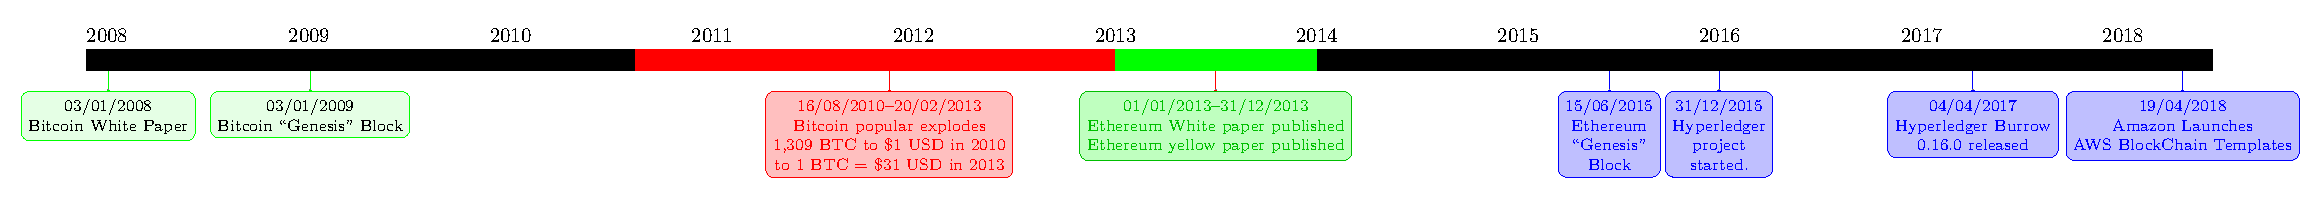
\includegraphics[width=1.2\linewidth]{Diagrams/advancedTimeline.pdf}
%\end{adjustbox}
%\caption{An example of server-blockchain architecture in a DAPP.}
%\label{fig:dappArc}
%\end{figure}



%%% Contain timeline
\vspace*{-0.25cm}
\subsubsection{Decentralized Applications}
%%% ClEAN TIHS UP LATER
	%A blockchain is a digitized, decentralized, public ledger of all cryptocurrency transactions. %To access websites on the Ethereum blockchain and use dapps a specialized browser is needed, or a browser plugin like \gls{MetaMask}. 
	Blockchain technology is revolutionizing the internet by establishing trust in shared data. \cite{book:bchainForDummies}.
	Additionally, transactions recorded on the blockchain are practically impossible to remove or change. 
	
	
	\begin{warpprint}
	\begin{figure}[ht]
	%\begin{adjustbox}{center,max width=1.1\textwidth}
	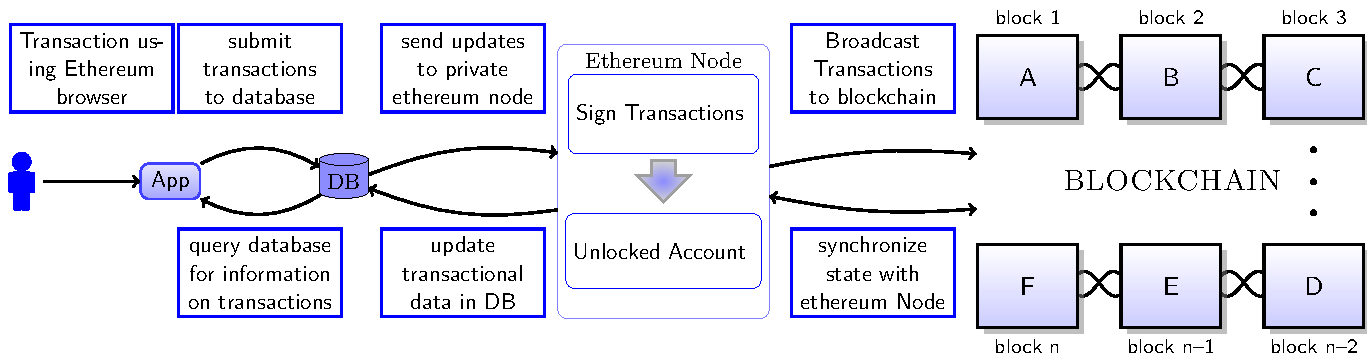
\includegraphics[width=1\linewidth]{Diagrams/blockchainInSimpleApp.pdf}
	%\end{adjustbox}
	\caption{An example of server-blockchain architecture in a DAPP.}
	\label{fig:DApp}
	\end{figure}
	\end{warpprint}
	
	\begin{warpHTML}
	\begin{figure}[ht]
	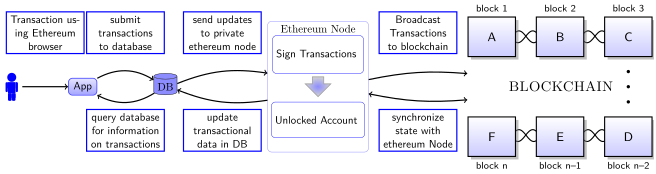
\includegraphics[width=1.2\linewidth]{Diagrams/blockchainInSimpleApp.svg}
	\caption{An example of server-blockchain architecture in a DAPP.}
	\label{fig:DApp}
	\end{figure}
	\end{warpHTML}
	
	A decentralized application, or \gls{DApp} are deployed on peer to peer networks such as \gls{Ethereum} or on the cloud \footnotemark. A decentralized system (peer to peer) has many advantages over a conventional centralized network including no single points of failure, cheaper distribution (servers are expensive), faster upload speeds. 
	\footnotetext[1]{Amazon recently started offering blockchain templates on Amazon Web Services (AWS). %\cite{ethereumWhitePaper:Online}
	}
	
	
	Despite, the obvious advantages of decentralized and \gls{blockchain} technologies,  a lack of resources for unpopular materials may result in prolonged downloads. An equivalent anecdote is a inadequately seeded torrent results in intolerable download speeds.  Whereas a traditional database only checks, writes and stores data once, a decentralized blockchain system require thousands of operations to write and store data, therefore the costs of maintaining a \gls{blockchain} are substantial higher and only justifiable with increased utility/security \cite{EthScale:Online}. 
	%\paragraph{Types of Blockchains}
	%\begin{itemize}
	%\item[---]  \textbf{Public blockchains} are large distributed networks that are run through a native token such as bitcoin or ether. Anyone can participate and the community maintains its open-source code. The two largest public blockchains are Ethereum and Bitcoin.%They’re open for anyone to participate at any level and have open-source code that their community maintains.
	% rewrite and add section about composer
	%\item[---] \textbf{Permissioned blockchains} define role based access control for individuals in the network and uses native tokens.  \gls{HyperLedger Composer}, an open-source framework for permissioned blockchains, is used for smart contracts and for blockchain application development \cite{hyperledgerComposer:Online}. One use case is an accounting system that calculates payment, while hiding that information from unrelated organizations.  % Their core code may or may not be open source.
	%\item[---] \textbf{Private blockchains}  membership is tightly controlled and lacks a native token. Useful for consortiums with trusted associates and exchanging confidential information, however, less powerful because it is supported by limited private resources.
	%\end{itemize}
	%\vspace*{-0.5cm}
	
	
	% Consider taking this part out, too detailed for the high level explaination.
	\paragraph{Public and Private Keys}
	 In a \gls{blockchain} system, any key holder can use their private key to sign a piece of data. This results in a signature.  
	  In a \gls{DApp}, this can be used for:
	 \begin{enumerate}
		\item Recovering the public key (ethereum account address) of the Author.
		\item Verify if the raw data is identical  using the Author's public key. 
	\end{enumerate}
	
	Blockchain technology has been proposed as a supplement to help consumers prove ownership of assets in digital systems.  Blockchains are fantastic public recordkeeping systems because they also can’t be backdated or changed without a recorded transaction. In theory, \glspl{blockchain} could transform untrustworthy transactions into distributed databases.
	%In order to sign something, a mathematical function is used to "sign" a piece of document/data. A digital signature of a document/data is a number generated using a private key. The private key has a corresponding public key. 
	
	
	
%	\begin{figure}[ht]
%	\centering
%	
\includegraphics[width=0.5\linewidth]{Diagrams/verifySig.png}
%	\caption{Illustrate how public and private keys are used to verify signatures}
%	\label{fig:verfSig}
%	\end{figure}
	
		 
% refer to medium article, and some other article highlighting the interest in private nodes, https://aws.amazon.com/partners/blockchain/
% https://blog.zeppelin.solutions/designing-the-architecture-for-your-ethereum-application-9cec086f8317
% https://aws.amazon.com/blogs/apn/introducing-aws-blockchain-partners/

%		To access websites on the Ethereum blockchain and use dapps a specialized browser is needed, or a plugin like metamask. 

\subsubsection{Smart Contracts}
%	\begin{minipage}[h]{0.5\linewidth}
		Traditional legal contracts are written to represent the contracting parties. In a smart contract, self-executing source code is used to automatic transactions that are publicly available on the blockchain \cite{ethereumWhitePaper:Online}.
		Furthermore, \glspl{smart contract} allow buyers and sellers exchange money, property, shares, or anything of value in a transparent, conflict-free way while avoiding the services of a middleman (See Figure \ref{fig:smartcontractcreation}). This allows validation of complex transactions swiftly while maintaining transparency. Although the benefits of using smart contracts are obvious, legal enforceability is difficult because "no central administering authority to decide a dispute" exists \cite{keyfindings:Online}. 


\begin{warpprint}
	\begin{figure}[ht]
		\centering
		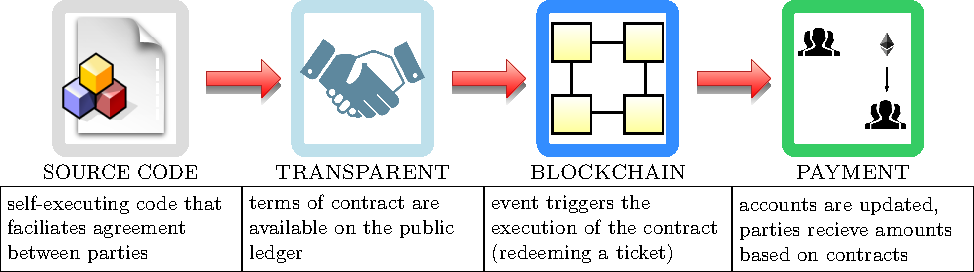
\includegraphics[width=1\linewidth]{Diagrams/smartContractsExp.pdf}
		\caption{Illustrating how a smart contract works}
		\label{fig:smartContracts}
	\end{figure}
\end{warpprint}

\begin{warpHTML}
	\begin{figure}[ht]
		\centering
		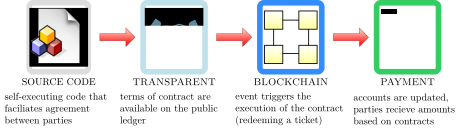
\includegraphics[width=1\linewidth]{Diagrams/smartContractsExp.svg}
		\caption{Illustrating how a smart contract works}
		\label{fig:smartContracts}
	\end{figure}
\end{warpHTML}

		In addition, irreversible and immutable transactions are a disadvantage that hackers can exploit. For example, an amateur coder killed the contract that allowed users to transfer Ether for the Parity \gls{Ethereum} Wallet, rendering 150 to 300 million dollars completely useless \cite{funnyJoke:Online}. Scrutinizing smart contracts and reducing bugs in production code is essential. An example of smart contract is available in Appendix A \ref{lst:label}.
		
		% Rewrite here.
		The desirable properties of a \gls{blockchain} such as integrity and immutability of data, e.g., transactions and
		smart contracts, require an active mining pool. In a proof of work consensus (POW) mechanism,  miners need to invest energy and resources,
		i.e. computational power, to participate in the consensus process and prevent tampering blocks. Additionally, miners are incentivized to run nodes that verify transactions through bitcoin or ether. %The investment must incentive miners to verify transactions and/or run nodes.%This investment has to be incentivized to prevent miners from not participating.
%	\end{minipage}
%	\begin{minipage}[h]{0.5\linewidth}
%		\begin{lstlisting}[language=Solidity,caption=Smart contract in Solidity]
%		// pragma is used to specifc version of Solidity
%		pragma solidity ^0.4.16;
%		contract HelloWorld {
%		 uint256 counter = 5; 
%		 //state variable we assigned earlier
%		 address owner = msg.sender; 
%		 //set owner as msg.sender
%		function add() public {  //increases counter by 1
%	  		counter++;
%		 }
%		 function subtract() public { //decreases counter by 1
%		  counter--;
%		 }
%		 function getCounter() public constant returns (uint256) {
%		  return counter;
%		 } 
%		 function kill() public { //self-destruct function, 
%		   if(msg.sender == owner) {
%		    selfdestruct(owner); 
%		   }
%		}
%		
%		// Fallback function
%		function () public payable {
%		
%		 }
%		\end{lstlisting}
%	\end{minipage}

%	\newpage
	
	
%	or internal processes such as supply chains, a private blockchain makes sense (data cannot be changed) and cryptographic auditing with known identities (public keys). For a trustless system, using a public blockchain makes the most sense. In comparsion, a permissioned blockchain is effective for limiting what can or cannot do, as well as prevent users from seeing other transactions they are not suppose to see.
	
	%Despite the slow speed of the public blockchain, innovations such as \gls{side chains} enable quick transactions and are used in blockchain game development \cite{loomNetwork:Online}. % 

\subsubsection{Advantages and Disadvantages of Decentralization }
Currently, centralized IT systems are vulnerable to "malicious attacks, software and hardware faults, human mistakes (e.g., software and hardware misconfigurations") \cite{5936160}. Decentralized systems have no single point of failure, improved security and are more transparent, however, efficient code is more important in smart contracts. As illustrated in Figure \ref*{fig:DApp} a \gls{blockchain}-server architecture model allows for developers to implement decentralized applications with smart contracts while maintaining the flexibility and simplicity of retrieving and sending information.	

\subsection{Objective}
The prominence of cryptocurrency and decentralized applications suggests usage of smart contracts will experience explosive growth.

\subsubsection{Problem}

Currently commonplace transactions require days to process and for parties verify correctness. For example to purchase houses, a plethora of steps are required, one must interactive with lawyers, real-estate agents, home inspector, buy insurance and shop for a mortgage. 

\subsubsection{Purpose}
Leveraging existing blockchain technologies can automatic the majority of steps and cut out the middlemen, resulting in buyers conversing directing with sellers.
Although smart contracts have immense potential to simplify transactions, issues such as limiting access to information, latency when updating (takes 10 minutes to write info to bitcoin blockchain), and immutability of translations (cannot undo fraudulent transfer of assets) must be addressed.
% See https://www.cs.auckland.ac.nz/research/groups/ssg/homepages/yu-cheng/ytu001_PhDThesis.pdf
% https://researchspace.auckland.ac.nz/handle/2292/22092
\subsection{Aims}
The aims of this project are to illustrate how a decentralized blockchain system can:
\begin{enumerate}
\item Reduce cost of transactions by at least 50\% from removing middlemen.
\item Improve transparency in software systems through augmented accessibility and understandability.
\item Increased security and greater enforceability of contractual obligations.
%1. Uses 15% less material to decrease cost and weight.
%2. Has improved efficiency by reducing the air gap by 10%.
%3. Has no reduction in its reliability or increase in its maintenance requirements. 
\end{enumerate}
\subsubsection{Limitations}

The regulatory uncertainty and impact of future regulations on \gls{blockchain} technologies such as \glspl{smart contract} will not be investigated. In addition, criminal usage of cryptocurrencies to avoid taxation and legal repercussions are beyond the scope of this report. In addition the impacts of quantum computing altering the validity of modern cryptography algorithms will not be investigated.
%The performance of the linear generator in extreme storm events will not be investigated as this
%cannot be accurately modeled using Airy linear wave theory. This project will be based on
%numerical simulations; no physical model will be tested to validate the results.

\newpage  

	
\section{Discussion}
As shown in 
		Figure \ref{fig:DApp} \gls{DApp}, a user's transactions on the application is publicly broadcasting to the blockchain. 
		Implementing architecture for blockchain 
		applications 
		
		\footnote{Although, server blockchain architecture with an abstraction layer resemble traditional applications, other approaches are available such as offline signing with a public node, and client-blockchain in serverless apps and leveraging cloud infrastructure.} 
		
		adds an third layer to the standard client-server architecture 	\footnote{ \textbf{Signing Transactions}: One approach involves interacting with the JSON RPC interface of the \gls{Ethereum} node from the application to perform all blockchain operations.}.
		 Disadvantages of blockchain data storage include difficult retrieving relevant information (without an abstraction layer, the entire blockchain or a single transaction is returned), users will experience latency before transactions are validated, 	\footnote{For bitcoin, it takes 10 minutes before blocks of transactions are validated because of the mining process.}
		 
		  and writing to the blockchain is relatively expensive compared to traditional systems. Usage of interfaces such as the JSON RPC and/or cloud hosting 
	 solutions	
	 	 serve as a abstraction layer allowing databases to load publicly available data on the blockchain
	 	 % rewrite later 
	 	 for more efficient user interactions with that information. 

\begin{warpprint}
\begin{figure}[ht]
\begin{adjustbox}{center,max width=1.1\textwidth}
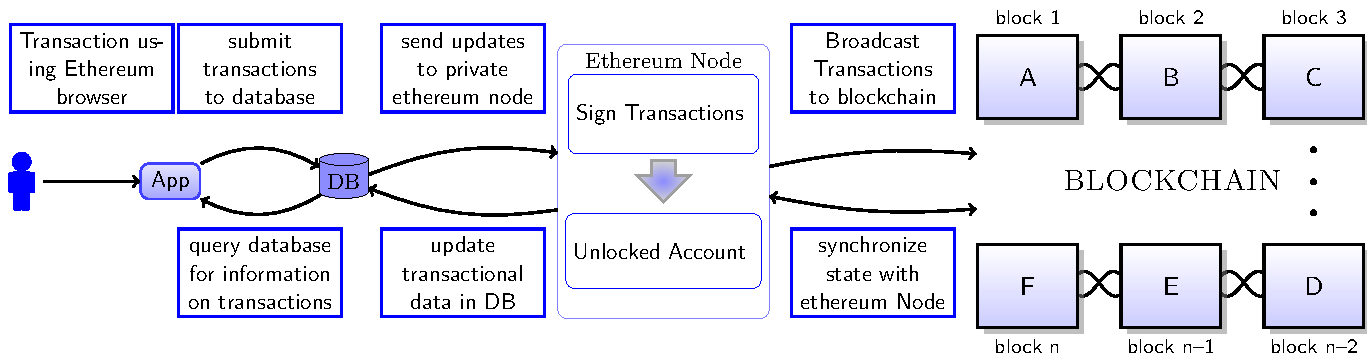
\includegraphics[width=1.2\linewidth]{Diagrams/blockchainInSimpleApp.pdf}
\end{adjustbox}
\caption{An example of server-blockchain architecture in a DAPP.}
\label{fig:DApp}
\end{figure}
\end{warpprint}

\begin{warpHTML}
\begin{figure}[ht]
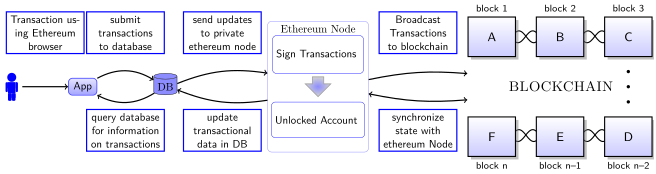
\includegraphics[width=1.2\linewidth]{Diagrams/blockchainInSimpleApp.svg}
\caption{An example of server-blockchain architecture in a DAPP.}
\label{fig:DApp}
\end{figure}
\end{warpHTML}

\begin{warpprint}
\begin{table}[]
\centering
\caption{Sample Decision Matrix for designing a blockchain system}
\arrayrulecolor{white}
\arrayrulewidth=1pt
\renewcommand{\arraystretch}{1.5}
\rowcolors[\hline]{3}{.!50!white}{}
\begin{tabular}{D E A B C }
\multicolumn{1}{l}{}      & \multicolumn{1}{c}{Existing Systems}    & \multicolumn{3}{c}{BlockChain Systems}                                                                                    \\
\multicolumn{1}{c}{Criteria}                 & \multicolumn{1}{c}{Centralized} & \multicolumn{1}{c}{Public} & \multicolumn{1}{c}{Permissioned} & \multicolumn{1}{c}{Private} \\
speed and latency         &                                         &                                       &                                             &                                        \\
scale and volume          &                                         &                                       &                                             &                                        \\
security and immutablity  &                                         &                                       &                                             &                                        \\
storage capacity          &                                         &                                       &                                             &                                        \\
transparency              &                                         &                                       &                                             &                                        \\
\multicolumn{1}{c}{Total} &                                         &                                       &                                             &                                       
\end{tabular}
\end{table}
\end{warpprint}

% HTML VERSION OF TABLE
\begin{warpHTML}

A generic message here? 

\begin{table}
\centering
\caption{My caption}
\begin{tabular}{cllll}
\multicolumn{1}{l}{}      & \multicolumn{1}{c}{Current Solution}    & \multicolumn{3}{c}{Alternative Solutions}                                                                                    \\
Criteria                  & \multicolumn{1}{c}{Centralized Systems} & \multicolumn{1}{c}{Public Blockchain} & \multicolumn{1}{c}{Permissioned Blockchain} & \multicolumn{1}{c}{Private Blockchain} \\
speed and latency         &                                         &                                       &                                             &                                        \\
scale and volume          &                                         &                                       &                                             &                                        \\
security and immutablity  &                                         &                                       &                                             &                                        \\
storage capacity          &                                         &                                       &                                             &                                        \\
transparency              &                                         &                                       &                                             &                                        \\
\multicolumn{1}{l}{Total} &                                         &                                       &                                             &                                       
\end{tabular}
\end{table}
\end{warpHTML}
\section{Conclusion}
Adopting JIRA has benefited ME by reducing response time, improving record keeping and sharpening communication. Although JIRA has benefited the organization by improving efficiency, lack of education resulting in underutilisation of dashboards and filters, occasional performance issues causing issue backlogs to pile up, and perceived unreliability for sending emails.  Agile software development methodologies such as Scrum and Kanban are supported by the JIRA suite of applications. JIRA has add-ons that extend functionality will complexity ranging from a single feature to full product.  Interestingly, when JIRA is integrated with Confluence usage of both applications will increase because jumping between application is quick and simple. \\

In order to streamline the adoption of \gls{Confluence}, usage intentions must be conveyed as well as detailed guidance on how to use it. Confluence is wiki software used to create knowledge bases, centralize information into a single system and for technical documentation. Useful features of Confluence include integration with \gls{JIRA}, word processing, and team collaboration.  Connecting JIRA and Confluence applications allows enable users to rapidly switch between applications.  Overall, JIRA and Confluence are software tools that improve productivity and organization within BTI IM.
 \section{Recommendations}
 
 
  
Obviously continued researching into \gls{blockchain} technologies is necessary as innovations such as permissioned blockchains such as \gls{HyperLedger Composer} and \gls{side chains} continue to address some shortcomings of blockchain. In trustless systems tampering or modification of transactional history is extremely difficult. This suggests that smart contracts can greatly improve transactions, however, issues including scalability, reversing fraudulent activity and reduction of contract deployment hinder mass adoption.

All computer programs have bugs, by limiting complexity of smart contracts,  using reliable standards highly audited packages, and using software security analyze tools risk can be greatly reduced. Continuing to monitor technology innovations such ever-increasing computational power is important to ensure cracking private keys remain uneconomical see Figure \ref{security:fig2}.

Provided a deterministic set of inputs and outputs, with computational verifiable conditions, using smart contracts is beneficial.
Increasing awareness about \gls{blockchain} technologies, so that the average person understands the limitations of smart contracts and in what situations they can be useful.

\newpage
%%%%%%%%%%%%%%%%%%%%%%%%%%%%%%%%%%%%%%%%%%%%%%
%%%% END Main Content %%%%%%%%%%%%%%%%%%%
%%%%%%%%%%%%%%%%%%%%%%%%%%%%%%%%%%%%%%%%%%%%%%

%%%%%%%%%%%%%%%%%%%%%%%%%%%%%%%%%%%%%%%%%%%%%%
%%% BACK MATTER, printing References %%%%%%%%%
%%%%%%%%%%%%%%%%%%%%%%%%%%%%%%%%%%%%%%%%%%%%%%
%\renewcommand\bibname{References} % Change bibliography to references

\section{References}
% nocite prints all references even if they were not used
\subsubsection*{Cited References}
 \printbibliography[heading=none,category=cited]

\subsubsection*{General References}
\printbibliography[heading=none,notcategory=cited,resetnumbers=true] 
\linespread{1}

\begin{appendices}
\section{Code Listings}
\lstinputlisting[
language   = C,
basicstyle = \ttfamily,
style		= default,
%frame      = single,
caption    = {Caesar Cipher for CSC 111},]
{Code/cipher.c}

\end{appendices}
\end{document}

%%%%%%%%%%%%%%%%
COMMON COMMANDS:
%%%%%%%%%%%%%%%%
% IMAGES
\begin{figure}[H]
	\begin{center}
		\includegraphics[width=0.6\textwidth]{RTL_SCHEM.png}
	\end{center}
	\caption{A screenshot of the RTL Schematics produced from the Verilog code.}
	\label{RTL}
\end{figure}

% SUBFIGURES IMAGES
\begin{figure}[H]
	\centering
	\subfloat[LED4 Period]{\label{fig:Per4}\includegraphics[width=0.4\textwidth]{period_led4.png}} \\                
	\subfloat[LED5 Period]{\label{fig:Per5}\includegraphics[width=0.4\textwidth]{period_led5.png}}
	\subfloat[LED6 Period]{\label{fig:Per6}\includegraphics[width=0.4\textwidth]{period_led6.png}}
	\caption{Period of LED blink rate captured by osciliscope.}
	\label{fig:oscil}
\end{figure}

% CITATIONS
\cite{CitationName}

% GLOSSARY ENTRY
\newglossaryentry{api}
{
	name={API},
	description={An Application Programming Interface (API) is a particular set
		of rules and specifications that a software program can follow to access and make use of the services and resources provided by another particular software program that implements that API},
	first={Application Programming Interface (API)},
	long={Application Programming Interface}
}
% INSERT SOURCE CODE
\lstinputlisting[
language=SQL,
basicstyle = \ttfamily,
style=			Oracle,
%frame      = single,
caption    = {Sample SQL Query},]
{Code/Data.sql}

% FANCY TABLE
\begin{table}
	\begin{center}
	\begin{tabular}{@{} l *4c @{}}
		\toprule
		\multicolumn{1}{c}{Models}    & A  & B  & C  & D  \\ 
		\midrule
		Model $X$ & X1 & X2 & X3 & X4 \\ 
		Model $Y$ & Y1 & Y2 & Y3 & Y4 \\
		\bottomrule
	\end{tabular}
	\caption{Caption}
	\end{center}
\end{table}

% TEXT TABLE
\begin{table}
	\begin{center}
		\begin{tabular}{|l|c|c|l|}
			x & x & x & x \\ \hline
			x & x & x & x \\
			x & x & x & x \\ \hline
		\end{tabular}
		\caption{Caption}
		\label{label}
	\end{center}
\end{table}

% MATHMATICAL ENVIRONMENT
$ 8 = 2 \times 4 $

% CENTERED FORMULA
\[  \]

% NUMBERED EQUATION
\begin{equation}

\end{equation}

% ARRAY OF EQUATIONS (The splat supresses the numbering)
\begin{align*}

\end{align*}

% NUMBERED ARRAY OF EQUATIONS
\begin{align}

\end{align}

% ACCENTS
\dot{x} % dot
\ddot{x} % double dot
\bar{x} % bar
\tilde{x} % tilde
\vec{x} % vector
\hat{x} % hat
\acute{x} % acute
\grave{x} % grave
\breve{x} % breve
\check{x} % dot (cowboy hat)

% FONTS
\mathrm{text} % roman
\mathsf{text} % sans serif
\mathtt{text} % Typewriter
\mathbb{text} % Blackboard bold
\mathcal{text} % Caligraphy
\mathfrak{text} % Fraktur

\textbf{text} % bold
\textit{text} % italic
\textsl{text} % slanted
\textsc{text} % small caps
\texttt{text} % typewriter
\underline{text} % underline
\emph{text} % emphasized

\begin{tiny}text\end{tiny} % Tiny
\begin{scriptsize}text\end{scriptsize} % Script Size
\begin{footnotesize}text\end{footnotesize} % Footnote Size
\begin{small}text\end{small} % Small
\begin{normalsize}text\end{normalsize} % Normal Size
\begin{large}text\end{large} % Large
\begin{Large}text\end{Large} % Larger
\begin{LARGE}text\end{LARGE} % Very Large
\begin{huge}text\end{huge}   % Huge
\begin{Huge}text\end{Huge}   % Very Huge

%   \Gls{agile} software development uses repeatable brief cycles called 
%   \glspl{sprint} that focus on short-term deliverables.
\begin{figure}
	\caption{A picture323}
\end{figure}
\begin{table}[H]
	\begin{center}
		\begin{tabular}{cccc}
			\toprule 
			Nucleus & \textit{I} & Natural Abundance / \% & Larmor Frequency @ 7T \\
			\midrule
			\rowcolor{black!20} \textsuperscript{1}H & \sfrac{1}{2} & 99.98 & 298.0 \\
			\textsuperscript{2}H & 1 & 0.02 & 45.7 \\
			\rowcolor{black!20} \textsuperscript{12}C & 0 & 98.90 & - \\
			\textsuperscript{13}C & \sfrac{1}{2} & 1.10 & 74.9 \\
			\rowcolor{black!20} \textsuperscript{14}N & 1 & 99.60 & 21.5 \\
			\textsuperscript{15}N & \sfrac{1}{2} & 0.40 & 30.2 \\
			\rowcolor{black!20} \textsuperscript{16}O & 0 & 99.96 & - \\
			\textsuperscript{17}O & \sfrac{1}{2} & 0.04 & 40.4 \\
			\bottomrule
		\end{tabular}
		\caption{Numbers232323}
	\end{center}
\end{table}

%%% COMPLETE TABLE EXAMPLE %%%%
\newcommand{\head}[1]{\textnormal{\textbf{#1}}}
\newcommand{\normal}[1]{\multicolumn{1}{l}{#1}}
\begin{table}
	\centering
	\begin{tabular}{@{}l*2{>{\textbackslash\ttfamily}l}%
			l<{Example text}l@{}}
		\toprule[1.5pt]
		& \multicolumn{2}{c}{\head{Input}}
		& \multicolumn{2}{c}{\head{Output}}\\
		& \normal{\head{Command}} & \normal{\head{Declaration}}
		& \normal{\head{Single use}} & \head{Combined}\\
		\cmidrule(lr){2-3}\cmidrule(l){4-5}
		\multirow{3}{*}{Family} &  textrm & rmfamily & \rmfamily & \\
		& textsf & sffamily & \sffamily & \\
		& texttt & ttfamily & \ttfamily & \\
		\cmidrule(lr){2-3}\cmidrule(lr){4-4}
		\multirow{2}{1.1cm}{Weight} & textbf & bfseries & \bfseries
		& \multirow{2}{1.8cm}{\sffamily\bfseries Bold and sans-serif} \\
		& textmd & mdseries & \mdseries & \\
		\cmidrule(lr){2-3}\cmidrule(lr){4-4}
		\multirow{4}{*}{Shape} & textit & itshape & \itshape & \\
		& textsl & slshape & \slshape &
		\multirow{2}{1.8cm}{\sffamily\slshape Slanted and sans-serif}\\
		& textsc & scshape & \scshape & \\
		& textup & upshape & \upshape & \\
		\cmidrule(lr){2-3}\cmidrule(lr){4-4}
		Default & textnormal & normalfont & \normalfont & \\
		\bottomrule[1.5pt]
	\end{tabular}
	\caption{\LaTeX\ font selection}
\end{table}
%%%%    END TABLE EXAMPLE   %%%%%

%%%% TABLE EXAMPLE %%%%
\newcolumntype{Y}{>{\raggedleft\arraybackslash}X}

\tcbset{tab1/.style={fonttitle=\bfseries\large,fontupper=\normalsize\sffamily,
		colback=yellow!10!white,colframe=red!75!black,colbacktitle=orange!40!white,
		coltitle=black,center title,freelance,frame code={
			\foreach \n in {north east,north west,south east,south west}
			{\path [fill=red!75!black] (interior.\n) circle (3mm); };},}}

\tcbset{tab2/.style={enhanced,fonttitle=\bfseries,fontupper=\normalsize\sffamily,
		colback=yellow!10!white,colframe=red!50!black,colbacktitle=yellow!40!white,
		coltitle=black,center title}}
\begin{table}
	\begin{tcolorbox}[tabularx={X||Y|Y|Y|Y||Y},title=My table]
		Group & One & Two & Three & Four & Sum\\\hline\hline
		Red & 1000.00 & 2000.00 & 3000.00 & 4000.00 & 10000.00\\\hline
		Green & 2000.00 & 3000.00 & 4000.00 & 5000.00 & 14000.00\\\hline
		Blue & 3000.00 & 4000.00 & 5000.00 & 6000.00 & 18000.00\\\hline\hline
		Sum & 6000.00 & 9000.00 & 12000.00 & 15000.00 & 42000.00
	\end{tcolorbox}
	\caption{Another Great Table}
\end{table}
\begin{table}
	\begin{tcolorbox}[tab1, tabularx={X||Y|Y|Y|Y||Y}]
		Group & One & Two & Three & Four & Sum\\\hline\hline
		Red & 1000.00 & 2000.00 & 3000.00 & 4000.00 & 10000.00\\\hline
		Green & 2000.00 & 3000.00 & 4000.00 & 5000.00 & 14000.00\\\hline
		Blue & 3000.00 & 4000.00 & 5000.00 & 6000.00 & 18000.00\\\hline\hline
		Sum & 6000.00 & 9000.00 & 12000.00 & 15000.00 & 42000.00
	\end{tcolorbox}
	\caption{Great Table}
\end{table}
\begin{table}
	\begin{tcolorbox}[tab2, tabularx={X||Y|Y|Y|Y||Y},title=My table]
		Group & One & Two & Three & Four & Sum\\\hline\hline
		Red & 1000.00 & 2000.00 & 3000.00 & 4000.00 & 10000.00\\\hline
		Green & 2000.00 & 3000.00 & 4000.00 & 5000.00 & 14000.00\\\hline
		Blue & 3000.00 & 4000.00 & 5000.00 & 6000.00 & 18000.00\\\hline\hline
		Sum & 6000.00 & 9000.00 & 12000.00 & 15000.00 & 42000.00
	\end{tcolorbox}
	\caption{Good Table}
\end{table}
%%%% END TABLE EXAMPLE %%%%

%ANOTHER TABLE EXAMPLE
\setlist{nolistsep}
\definecolor{green}{HTML}{66FF66}
\definecolor{myGreen}{HTML}{009900}

%\renewcommand{\familydefault}{\sfdefault}


\begin{table}
	\begin{center}
		\begin{tabularx}{\textwidth}[t]{XX}
			\arrayrulecolor{green}\hline
			\textbf{\textcolor{myGreen}{Goal 1 Eradicate Extreme Poverty}} & \\
			\hline
			Target 1.A Halve, between 1990 and 2015, the proportion of the people whose income is less than \$1 a day. & 
			\begin{minipage}[t]{\linewidth}%
				\begin{itemize}
					\item[1.1] Proportion of population below \$1 purchasing power parity (PPP) a day$^a$
					\item[1.2] Poverty Gap ratio [incidence x depth of poverty]
					\item[1.3] Share of the poorest quintile in national consumption
				\end{itemize} 
			\end{minipage}\\
			
			\arrayrulecolor{black}\hline
			
			Target 1.B Achieve full and productive employment and decent work for all, including women and young people &
			\begin{minipage}[t]{\linewidth}%
				\begin{itemize}
					\item[1.4] Growth of GDP per person employed 
					\item[1.5] Employment to population ratio
					\item[1.6] Proportion of employed people living below \$1 (PP) a day
					\item[1.7] Proportion of own-account and contribution family workers in total employment
				\end{itemize} 
			\end{minipage}\\
			
			\hline
			
			Target 1.C Halve, between 1990 and 2015, the proportion of people who suffer from hunger &
			\begin{minipage}[t]{\linewidth}%
				\begin{itemize}
					\item[1.8] Prevalence of underweight children under five years of age
					\item[1.9] Proportion of population below minimum level of dietary energy consumption
				\end{itemize}
			\end{minipage}\\
			
			\arrayrulecolor{green}\hline
			\textbf{\textcolor{myGreen}{Goal 2 Achieve universal primary education}} \\
			\hline
			
			Target 2.A Ensure that by 2015 children everywhere, boy and girls alike, will be able to complete a full course of primary schooling. &
			\begin{minipage}[t]{\linewidth}%
				\begin{itemize}
					\item[2.1] Net enrollment ratio in primary education
					\item[2.2] Proportion of pupils starting grade 1 who reach last grade of primary education
					\item[2.3] Literacy rate of 15- to 24-year-olds, women and men
				\end{itemize}
			\end{minipage}\\
			
			\hline
			\multicolumn{2}{l}{%
				\textbf{\textcolor{myGreen}{Goal 3 Promote gender equality and empower women}}} \\
			\hline
			
			Target 3.A Eliminate gender disparity in primary and secondary education, preferably by 2005, and in all levels of education no later than 2015 &
			\begin{minipage}[t]{\linewidth}%
				\begin{itemize}
					\item[3.1] Ratios of girls to boys in primary, secondary and tertiary education
					\item[3.2] Share of women in wage employment in the non-agricultural sector.
				\end{itemize} 
			\end{minipage}
		\end{tabularx}
	\end{center}
	\caption{Great table to use}
\end{table}
% END ANOTHER TABLE EXAMPLE
\begin{figure}
	\caption{Another picture2323}
\end{figure}


\lstinputlisting[
language=SQL,
basicstyle = \ttfamily,
style=			Oracle,
caption    = {Sample SQL Query},]
{Code/Data.sql}	

\begin{table}
	\begin{center}
		\begin{tabular}{ |l|l|l| }
			\hline
			\multicolumn{3}{ |c| }{Team sheet} \\
			\hline
			Goalkeeper & GK & Paul Robinson \\ \hline
			\multirow{4}{*}{Defenders} & LB & Lucas Radebe \\
			& DC & Michael Duburry \\
			& DC & Dominic Matteo \\
			& RB & Didier Domi \\ \hline
			\multirow{3}{*}{Midfielders} & MC & David Batty \\
			& MC & Eirik Bakke \\
			& MC & Jody Morris \\ \hline
			Forward & FW & Jamie McMaster \\ \hline
			\multirow{2}{*}{Strikers} & ST & Alan Smith \\
			& ST & Mark Viduka \\
			\hline
		\end{tabular}
	\end{center}
	\caption{Table Title}
\end{table}

\begin{table} 
	\begin{center}
		\begin{tabular}{cccccccc} \toprule
			{$m$} & {$\Re\{\underline{\mathfrak{X}}(m)\}$} & {$-\Im\{\underline{\mathfrak{X}}(m)\}$} & {$\mathfrak{X}(m)$} & {$\frac{\mathfrak{X}(m)}{23}$} & {$A_m$} & {$\varphi(m)\ /\ ^{\circ}$} & {$\varphi_m\ /\ ^{\circ}$} \\ \midrule
			1  & 16.128 & +8.872 & 16.128 & 1.402 & 1.373 & -146.6 & -137.6 \\
			2  & 3.442  & -2.509 & 3.442  & 0.299 & 0.343 & 133.2  & 152.4  \\
			3  & 1.826  & -0.363 & 1.826  & 0.159 & 0.119 & 168.5  & -161.1 \\
			4  & 0.993  & -0.429 & 0.993  & 0.086 & 0.08  & 25.6   & 90     \\ \midrule
			5  & 1.29   & +0.099 & 1.29   & 0.112 & 0.097 & -175.6 & -114.7 \\
			6  & 0.483  & -0.183 & 0.483  & 0.042 & 0.063 & 22.3   & 122.5  \\
			7  & 0.766  & -0.475 & 0.766  & 0.067 & 0.039 & 141.6  & -122   \\
			8  & 0.624  & +0.365 & 0.624  & 0.054 & 0.04  & -35.7  & 90     \\ \midrule
			9  & 0.641  & -0.466 & 0.641  & 0.056 & 0.045 & 133.3  & -106.3 \\
			10 & 0.45   & +0.421 & 0.45   & 0.039 & 0.034 & -69.4  & 110.9  \\
			11 & 0.598  & -0.597 & 0.598  & 0.052 & 0.025 & 92.3   & -109.3 \\ \bottomrule
		\end{tabular}
	\end{center}
	\caption{Table Title}
\end{table}